\documentclass[xga]{xdvislides}
\usepackage[landscape]{geometry}
\usepackage{graphics}
\usepackage{graphicx}
\usepackage{colordvi}
\usepackage{fancyvrb}

\fvset{fontfamily=courier,commandchars=\\\{\}}

\begin{document}
\setfontphv

%%% Headers and footers
\lhead{\slidetitle}                               % default:\lhead{\slidetitle}
\chead{CS615 - Aspects of System Administration}% default:\chead{\relax}
\rhead{Slide \thepage}                       % default:\rhead{\sectiontitle}
\lfoot{\Gray{Configuration Management}}% default:\lfoot{\slideauthor}
\cfoot{\relax}                               % default:\cfoot{\relax}
\rfoot{\Gray{\today}}

\newcommand{\smallish}{\fontsize{16}{16}\selectfont}

\vspace*{\fill}
\begin{center}
	\Hugesize
		CS615 - Aspects of System Administration\\ [1em]
		Configuration Management\\ [1em]
	\hspace*{5mm}\blueline\\ [1em]
	\Normalsize
		Department of Computer Science\\
		Stevens Institute of Technology\\
		Jan Schaumann\\
		\verb+jschauma@stevens-tech.edu+
		\verb+https://www.cs.stevens.edu/~jschauma/615A/+
\end{center}
\vspace*{\fill}

\subsection{To the backups!}
\vspace*{\fill}
\begin{center}
	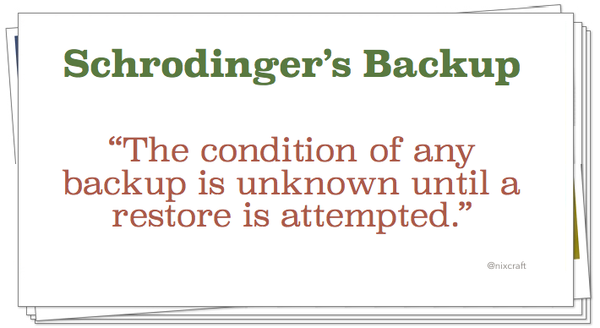
\includegraphics[scale=0.8]{pics/schrodinger.eps}
\end{center}
\vspace*{\fill}

\subsection{HW Review}
\\

\vspace{.5in}
\Huge
\begin{center}
Use your words!
\end{center}
\Normalsize

\subsection{Entropy is the Enemy}
\vfill
\Huge
\begin{center}
The entropy of an isolated system never decreases.
\end{center}
\Normalsize
\vfill

\subsection{Entropy is the Enemy}
A static system is a useless system.
A useful system is being used.
\vspace{.5in}
\begin{itemize}
	\item data is processed; files are created, modified, removed
	\item software is added, upgraded, removed
	\item systems are created, copied, decommissioned
	\item instances / containers are even more short-lived,
		coming into existence and disappearing again as needed
\end{itemize}

\subsection{Single Systems are Fragile}
Individual systems created and configured by hand are
fragile.  Our processes need to be repeatable,
automated, reliable. \\

Recall previous lectures:

\begin{itemize}
	\item OS installation
	\item package management
	\item multi-user basics
	\item automation
	\item recovery / restores
\end{itemize}

\subsection{Reproducable}
\vspace*{\fill}
\begin{center}
	
\includegraphics[scale=0.3]{pics/throw.eps} \\
	\vspace*{\fill}
	{\em ``Never trust a computer you can't throw out the
window.''} -- Woz
\end{center}

\subsection{Evolution of Configuration Management}
``I set up a server over here to do X.  Replicate that
setup on all the others.'' \\

\subsection{Evolution of Configuration Management}
``I set up a server over here to do X.  Replicate that
setup on all the others.'' \\

``I know how to do this!  Watch me!'' \\
\begin{verbatim}
$ ssh root@server1
# rsync -e ssh -avz / server2:/
\end{verbatim}
\vspace{.5in}
``{\tt /etc}?  What's that?''

\subsection{Evolution of Configuration Management}
\\

\vspace{.5in}
\Huge
        \begin{tabular}{ l | l | l }
        & shareable content & unshareable content \\
        \hline
        static data & {\tt /usr} & {\tt /boot} \\
        & {\tt /opt} & {\tt /etc} \\
        \hline
        variable data & {\tt /home} & {\tt /tmp} \\
        & {\tt /var/mail} & {\tt /var/run} \\
        \hline
        \end{tabular}
\Normalsize

\subsection{Every Sysadmin ever...}
\begin{enumerate}
	\item {\tt scp(1)}
\end{enumerate}

\subsection{Every Sysadmin ever...}
\begin{enumerate}
	\item {\tt scp(1)}
	\item {\tt rsync(1)}
\end{enumerate}

\subsection{Every Sysadmin ever...}
\begin{enumerate}
	\item {\tt scp(1)}
	\item {\tt rsync(1)}
	\item some sort of parallel {\tt ssh(1)} of the above
\end{enumerate}

\subsection{Every Sysadmin ever...}
\begin{enumerate}
	\item {\tt scp(1)}
	\item {\tt rsync(1)}
	\item some sort of parallel {\tt ssh(1)} of the above
	\item switch to {\em pull}
\end{enumerate}

\subsection{Every Sysadmin ever...}
\begin{enumerate}
	\item {\tt scp(1)}
	\item {\tt rsync(1)}
	\item some sort of parallel {\tt ssh(1)} of the above
	\item switch to {\em pull}
	\item add mutual authentication
\end{enumerate}

\subsection{Every Sysadmin ever...}
\begin{enumerate}
	\item {\tt scp(1)}
	\item {\tt rsync(1)}
	\item some sort of parallel {\tt ssh(1)} of the above
	\item switch to {\em pull}
	\item add mutual authentication
	\item but effectively ignore mismatches, because doing things the right way is difficult and inconvenient
\end{enumerate}

\subsection{Every Sysadmin ever...}
\begin{enumerate}
	\item {\tt scp(1)}
	\item {\tt rsync(1)}
	\item some sort of parallel {\tt ssh(1)} of the above
	\item switch to {\em pull}
	\item add mutual authentication
	\item but effectively ignore mismatches, because doing things the right way is difficult and inconvenient
	\item switch to {\em push} with remote d\ae mon
\end{enumerate}

\subsection{Every Sysadmin ever...}
\begin{enumerate}
	\item {\tt scp(1)}
	\item {\tt rsync(1)}
	\item some sort of parallel {\tt ssh(1)} of the above
	\item switch to {\em pull}
	\item add mutual authentication
	\item but effectively ignore mismatches, because doing things the right way is difficult and inconvenient
	\item switch to {\em push} with remote d\ae mon
	\item write an inventory database
\end{enumerate}

\subsection{Every Sysadmin ever...}
\begin{enumerate}
	\item {\tt scp(1)}
	\item {\tt rsync(1)}
	\item some sort of parallel {\tt ssh(1)} of the above
	\item switch to {\em pull}
	\item add mutual authentication
	\item but effectively ignore mismatches, because doing things the right way is difficult and inconvenient
	\item switch to {\em push} with remote d\ae mon
	\item write an inventory database
	\item deploy a well-known CM system
\end{enumerate}

\subsection{Every Sysadmin ever...}
\begin{enumerate}
	\item {\tt scp(1)}
	\item {\tt rsync(1)}
	\item some sort of parallel {\tt ssh(1)} of the above
	\item switch to {\em pull}
	\item add mutual authentication
	\item but effectively ignore mismatches, because doing things the right way is difficult and inconvenient
	\item switch to {\em push} with remote d\ae mon
	\item write an inventory database
	\item deploy a well-known CM system
\end{enumerate}
\vspace{.25in}

Finally: find something it can't do, goto 1.

\subsection{Base configuration vs. service definition}
Your servers have {\em unique}, yet predictable
properties.  E.g.:

\begin{itemize}
	\item network configuration
	\item critical services: DNS, NTP, Syslog 
	\item minimum OS / software version
	\item user management
	\item common service configuration (e.g. {\tt sshd(8)})
	\item ...
\end{itemize}

\subsection{Base configuration vs. service definition}
Different sets of servers have {\em shared}
properties.  For example, consider an HTTP server:

\begin{itemize}
	\item minimum server software
	\item appropriate TLS specification
	\item shared TLS certificate and key
	\item database configuration
	\item static content (HTML / JS / CSS files)
	\item ...
\end{itemize}

\subsection{Pets vs. Cattle}
``Pets'':
\begin{itemize}
	\item unique, cheerful hostnames
	\item single systems grown over time, lovingly configured by hand
	\item when sick, everybody is very concerned
	\item slowly nursed back to life
\end{itemize}
\vspace{.25in}
``Cattle'':
\begin{itemize}
	\item predictable, boring hostnames
	\item almost identical to all others
	\item centrally managed, easy to recreate
	\item when sick, they get taken out back and shot
	\item quickly replaced by another
\end{itemize}

\subsection{Service definitions}
\small
\begin{verbatim}
class syslog {
  include cron
  include logrotate
  package {
    'syslog−ng' :
      ensure  => latest ,
      require => Service['syslog−ng'];
  }
  service {
    'syslog−ng' :
      ensure => running ,
      enable => true;
  }
  file {
    '/etc/syslog−ng/syslog−ng.conf':
      ensure  => file,
      source  => 'puppet:///syslog/syslog−ng.conf',
      mode    => '0644',
      owner   => 'root',
      group   => 'root',
      require => Package['syslog-ng'],
      notify  => Service['syslog-ng'];

    '/etc/logrotate.d/syslog-ng':
      ensure  => file,
      source  => 'puppet:///syslog/logrotate-syslog−ng',
      mode    => '0644',
      owner   => 'root',
      group   => 'root',
      require => Package['logrotate'];
  }
}
\end{verbatim}
\Normalsize

\subsection{Service definitions}
\smallish
\begin{verbatim}
package "ldap-utils" do
  action :upgrade
end

template "/etc/ldap.conf" do
  source "ldap.conf.erb"
  mode   00644
  owner  "root"
  group  "root"
end

%w{ account auth password session }.each do |pam|
  cookbook_file "/etc/pam.d/common-#{pam}" do
    source   "common-#{pam}"
    mode     00644
    owner    "root"
    group    "root"
    notifies :restart, resources(:service => "ssh"), :delayed
  end
end
\end{verbatim}
\Normalsize

\subsection{Service definitions}
\smallish
\begin{verbatim}
bundle agent sshd(parameter) {
    files:
        "/tmp/sshd_config.tmpl"
            perms     => mog("0600","root","root"),
            copy_from => secure_cp("/templates/etc/ssh/sshd_config",
                                   "cf-master.example.com");

        "/etc/ssh/sshd_config"
            perms     => mog("0600","root","root"),
            create    => true,
            edit_line => expand_template("/tmp/sshd_config.tmpl"),
            classes   => if_repaired("restart_sshd");

    commands:
        restart_sshd::
            "/etc/rc.d/sshd restart"
}
\end{verbatim}
\Normalsize

\subsection{CM Requirements}
\begin{itemize}
	\item software installation
\end{itemize}

\subsection{CM Requirements}
\begin{itemize}
	\item software installation
	\item service management / supervising
\end{itemize}

\subsection{CM Requirements}
\begin{itemize}
	\item software installation
	\item service management / supervising
	\item file permissions / ownership
\end{itemize}

\subsection{CM Requirements}
\begin{itemize}
	\item software installation
	\item service management / supervising
	\item file permissions / ownership
	\item static files
\end{itemize}

\subsection{CM Requirements}
\begin{itemize}
	\item software installation
	\item service management / supervising
	\item file permissions / ownership
	\item static files
	\item host-specific data
\end{itemize}

\subsection{CM Requirements}
\begin{itemize}
	\item software installation
	\item service management / supervising
	\item file permissions / ownership
	\item static files
	\item host-specific data
\end{itemize}
\vspace{.25in}
\begin{itemize}
	\item command-execution
\end{itemize}

\subsection{CM Requirements}
\begin{itemize}
	\item software installation
	\item service management / supervising
	\item file permissions / ownership
	\item static files
	\item host-specific data
\end{itemize}
\vspace{.25in}
\begin{itemize}
	\item command-execution
	\item data collection
\end{itemize}

\subsection{One more layer of abstraction...}
\vspace{.5in}

The objective of a CM system is not to {\em make
changes} on a system. \\

\vspace{.5in}

The objective of a CM system is to {\em assert state}.

\subsection{CM States}
\vspace*{\fill}
\begin{center}
	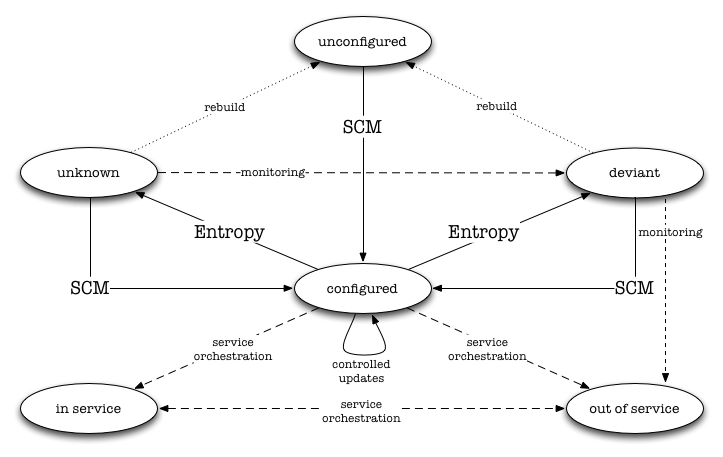
\includegraphics[scale=0.7]{pics/host-states.eps} \\
\end{center}
\vspace*{\fill}

\subsection{Circles around things}
Group your resources into {\em sets}. \\
\vspace{.5in}

\begin{itemize}
	\item functional groupings
	\item services
	\item users
	\item hosts
\end{itemize}

\subsection{Circles around things}
\vspace*{\fill}
\begin{center}
	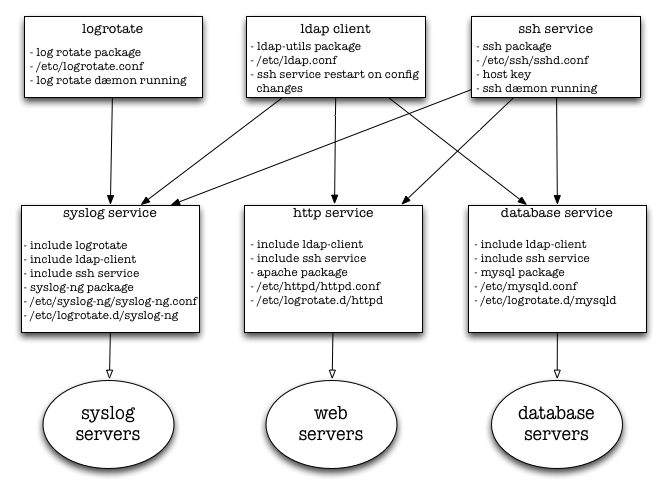
\includegraphics[scale=0.7]{pics/change-sets.eps} \\
\end{center}
\vspace*{\fill}

\subsection{Circles around things}
\vspace*{\fill}
\begin{center}
	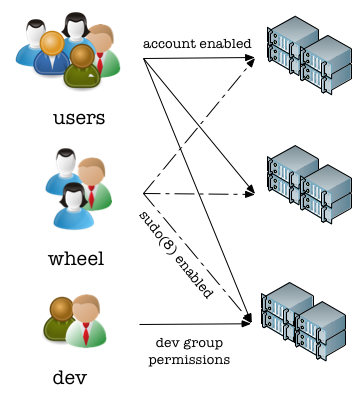
\includegraphics[scale=0.7]{pics/groups-machines.eps} \\
\end{center}
\vspace*{\fill}

\subsection{Circles around things}
\vspace*{\fill}
\begin{center}
	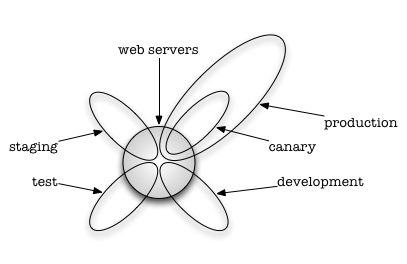
\includegraphics[scale=1.0]{pics/host-sets.eps} \\
\end{center}
\vspace*{\fill}

\subsection{CMs configure complex systems}
CM systems are complex themselves. \\
\vspace{.25in}

CM systems are inherently trusted. \\
\vspace{.25in}

CM systems can break everything.  To the degree that
you can't unbreak things afterwards. \\
\vspace{.5in}

Consider:
\begin{itemize}
	\item staged rollout of change sets
	\item automated error detection and rollback
	\item self-healing properties
	\item authentication and privilege
\end{itemize}


\subsection{Idempotence}
CM systems assert state.  For this, all operations
must be {\em idempotent}. \\
\vspace{.5in}

\begin{displaymath}
f(f(x)) \equiv f(x)
\end{displaymath}

\begin{displaymath}
| |-1| | \equiv |-1|
\end{displaymath}

\subsection{Idempotence}
CM systems assert state.  For this, all operations
must be {\em idempotent}. \\
\vspace{.5in}

\begin{displaymath}
f(f(x)) \equiv f(x)
\end{displaymath}

\begin{displaymath}
| |-1| | \equiv |-1|
\end{displaymath}

\begin{verbatim}
$ cd etc
\end{verbatim}

\subsection{Idempotence}
CM systems assert state.  For this, all operations
must be {\em idempotent}. \\
\vspace{.5in}

\begin{displaymath}
f(f(x)) \equiv f(x)
\end{displaymath}

\begin{displaymath}
| |-1| | \equiv |-1|
\end{displaymath}

\begin{verbatim}
$ cd etc                                            # not idempotent
$ rm resolv.conf
\end{verbatim}

\subsection{Idempotence}
CM systems assert state.  For this, all operations
must be {\em idempotent}. \\
\vspace{.5in}

\begin{displaymath}
f(f(x)) \equiv f(x)
\end{displaymath}

\begin{displaymath}
| |-1| | \equiv |-1|
\end{displaymath}

\begin{verbatim}
$ cd etc                                            # not idempotent
$ rm resolv.conf                                    # idempotent
$ echo "nameserver 192.168.0.1" > resolv.conf
\end{verbatim}

\subsection{Idempotence}
CM systems assert state.  For this, all operations
must be {\em idempotent}. \\
\vspace{.5in}

\begin{displaymath}
f(f(x)) \equiv f(x)
\end{displaymath}

\begin{displaymath}
| |-1| | \equiv |-1|
\end{displaymath}

\begin{verbatim}
$ cd etc                                            # not idempotent
$ rm resolv.conf                                    # idempotent
$ echo "nameserver 192.168.0.1" > resolv.conf       # idempotent
$ echo "nameserver 192.168.0.2" >> resolv.conf
\end{verbatim}

\subsection{Idempotence}
CM systems assert state.  For this, all operations
must be {\em idempotent}. \\
\vspace{.5in}

\begin{displaymath}
f(f(x)) \equiv f(x)
\end{displaymath}

\begin{displaymath}
| |-1| | \equiv |-1|
\end{displaymath}

\begin{verbatim}
$ cd etc                                            # not idempotent
$ rm resolv.conf                                    # idempotent
$ echo "nameserver 192.168.0.1" > resolv.conf       # idempotent
$ echo "nameserver 192.168.0.2" >> resolv.conf      # not idempotent
$ chown root:wheel resolv.conf
\end{verbatim}

\subsection{Idempotence}
CM systems assert state.  For this, all operations
must be {\em idempotent}. \\
\vspace{.5in}

\begin{displaymath}
f(f(x)) \equiv f(x)
\end{displaymath}

\begin{displaymath}
| |-1| | \equiv |-1|
\end{displaymath}

\begin{verbatim}
$ cd etc                                            # not idempotent
$ rm resolv.conf                                    # idempotent
$ echo "nameserver 192.168.0.1" > resolv.conf       # idempotent
$ echo "nameserver 192.168.0.2" >> resolv.conf      # not idempotent
$ chown root:wheel resolv.conf                      # idempotent
$ chmod 0644 resolv.conf                            # idempotent
\end{verbatim}

\subsection{Convergence and Eventual Consistency}
Note: idempotence does not guarantee efficiency! \\
\vspace{.5in}

CM systems should ensure changes are:
\begin{enumerate}
	\item idempotent (well, that part's on you)
	\item only applied if needed
	\item eventually consistent
\end{enumerate}
\vspace{.5in}

This often requires complexity (oh no!), coordination
with and awareness of other systems.  {\em Service
Orchestration} has developed as a separate, related
discipline to help address this.

\subsection{Distributed Systems}
CM systems are {\em distributed} systems.  As such,
they are subject to the CAP Theorem: \\

{\em Consistency}: all systems managed by the CM are
consistent within their respective service definition.
\\

{\em Availability}: the services managed by the CM are
kept available, even if no further updates or change
sets can be retrieved. \\

{\em Partition tolerance}: the CM system can (continue
to) operate despite interruptions between its
components; e.g. intermediate (coordinated) changes
are not required.

\subsection{More than just servers...}
Configuration Management is not just for servers.  You
also need to manage configurations for:
\vspace{.25in}

\begin{itemize}
	\item network equipment
	\item load balancers
	\item containers
	\item ...
\end{itemize}

\subsection{Overlap with other systems}
\vspace*{\fill}
\begin{center}
	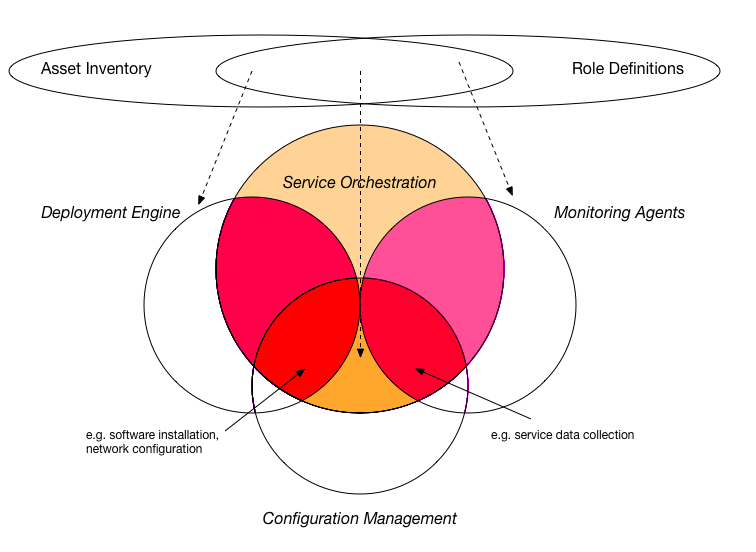
\includegraphics[scale=0.6]{pics/cm-overlap.eps} \\
\end{center}
\vspace*{\fill}


\subsection{Reading}

Additional topics to research:
\begin{itemize}
	\item Service Orchestration
	\item Continuous Deployment / Continuous Integration
	\item Infrastructure as Code
	\item Information Technology Infrastructure Library (ITIL)
\end{itemize}
\vspace{.25in}

Relevant links:
\begin{itemize}
	\item {\tt http://www.infrastructures.org/bootstrap/recovery.shtml}
	\item {\tt https://is.gd/paZ7qu}
	\item {\tt https://blog.engineyard.com/2014/pets-vs-cattle}
	\item {\tt http://markburgess.org/blog\_cap.html}
	\item {\tt http://markburgess.org/blog\_cap2.html}
	\item {\tt https://aws.amazon.com/opsworks/chefautomate/}
	\item {\tt https://puppet.com/product/managed-technology/aws}
\end{itemize}

\end{document}
